\chapterimage{heading_stats}
\opensidepicturearea
\chapter{Estatística}

\section{O que é Estatística}

Estatística é um conjunto de técnicas que permite, de tal forma, planejar, coletar, organizar, descrever, analisar e interpretar \emphasis{dados} de estudos ou experimentos, realizados em qualquer área do conhecimento.

Denomina-se por dados um (ou mais) conjunto de valores numéricos ou não.

\begin{example}\hfill
	\begin{itemize}
		\item \emphasis{Número de Tratores}\\
		\noindent 2, 0, 1, 2, 0, 3, 5, 1, 1, 2, 2, 3, $\dots$
		
		\item \emphasis{Uso do Solo}\\
		\noindent Agricultura, pastagem, vegetação nativa, agricultura, $\dots$
	\end{itemize}
\end{example}
	
\section{Principais Fases do Método Estatístico}
	
\begin{itemize}
	\item \emphasis{Definição do problema:} A primeira fase do trabalho estatístico consiste em uma definição do problema a ser estudado. Saber aquilo que se pretende pesquisar é o mesmo que definir corretamente o problema.

	\item \emphasis{Planejamento:} Nesta fase, a preocupação maior reside na escolha das perguntas, bem como sua correta formulação. É nessa fase que será definido o cronograma e o tipo de levantamento: \emphasis{censitário} ou por \emphasis{amostragem}.

	\item \emphasis{Coleta dos dados:} O terceiro passo é essencialmente operacional, compreendendo a coleta das informações propriamente ditas.

	\item \emphasis{Apuração dos dados:} É um trabalho de condensação e de tabulação dos dados, que chegam ao analista de forma desorganizada.

	\item \emphasis{Apresentação dos dados:} A apresentação ou exposição dos dados consiste na quinta fase do método estatístico.

	\item \emphasis{Análise e interpretação:} A última fase é a mais importante e também a mais delicada. Nesta etapa, o interesse maior reside em tirar conclusões que auxiliem o pesquisador a resolver seu problema.
\end{itemize}
	
\section{Alguns Conceitos Estatísticos}
	
\begin{itemize}
	\item \emphasis{Dados Brutos:} é uma sequência de valores não organizados, obtidos diretamente da observação de um fenômeno.	
	\begin{example}\hfill
	
		\emphasis{Peso}: 82, 74, 59, 62, 68
	\end{example}
		
	\item \emphasis{Rol:} é uma sequência ordenada de dados brutos.
	\begin{example}\hfill
	
		\emphasis{Peso}: 59, 62, 68, 74, 82
	\end{example}
		
	\item \emphasis{População:} é o conjunto de indivíduos (ou objetos), tendo pelo menos uma característica em comum observável.
	\begin{example}\hfill
		
		Alunos da Universidade Estadual de Goiás.
	\end{example}
		
	\item \emphasis{Amostra:} subconjunto não vazio da população.
	\begin{example}\hfill
	
		620 alunos da UEG.
	\end{example}
		
	\item \emphasis{Parâmetro:} é uma medida numérica que descreve uma característica da população.
	\begin{example}\hfill
		
		Altura média da população (\textbf{A}).
	\end{example}
		
	\item \emphasis{Estimador:} é qualquer função das observações.
	\begin{example}\hfill
	
		Seja
		\[
			\overline{A}=\frac{\displaystyle\sum_{i=1}^n A_i}{n}=\frac{A_1+A_2+\cdots+A_n}{n}\text{,}
		\]
		onde $A_i$ é a altura do $i$-ésimo individuo e $n$ é o número de indivíduos na amostra.
	\end{example}
	
	\item \emphasis{Estimativa:} é o valor numérico determinado pelo estimador.
	\begin{example}\hfill
	
		A altura média de 1,70m.
	\end{example}
		
	\item \emphasis{Censo:} é uma avaliação direta de um parâmetro, utilizando-se todos os componentes da população.
		
	\item \emphasis{Estimação:} é uma avaliação indireta de um parâmetro, com base em um estimador.
\end{itemize}

\subsection{Propriedades Principais do Censo}

\begin{itemize}
	\item Admite erro processual zero.
	\item Confiabilidade 100\%.
	\item É caro e lento.
	\item É quase sempre desatualizado.
\end{itemize}

\subsection{Propriedades Principais da Estimação}

\begin{itemize}
	\item Admite erro processual positivo.
	\item Confiabilidade menor que 100\%.
	\item É barata e Rápida.
	\item É quase sempre atualizada.
\end{itemize}

\section{Introdução a Técnicas de Amostragem}

Em estatística, em geral não observamos todos os elementos da população, pois isso pode demorar muito tempo, ter um custo econômico muito alto ou, até mesmo ser impossível. Então para resolver este empecilho, observamos uma amostra.

Para que se tenha uma amostra confiável, é necessário garantir que ela seja representativa da população, ou seja, a amostra deve possuir as mesmas características básicas da população de interesse.

A obtenção de soluções adequadas para o problema de amostragem exige, em geral, muito bom-senso e experiência. Entretanto existem dois métodos para a composição da amostra: \emphasis{Probabilístico} e \emphasis{Não-Probabilístico}.

\subsection{Amostragem Não-Probabilística}

São amostras em que há uma escolha deliberada dos elementos da amostra. Dentre elas destacamos:
\begin{itemize}
	\item \emphasis{Amostragem Acidental}: Trata-se de uma amostra formada por aqueles elementos que vão aparecendo, que são possíveis de se obter até completar o número de elementos na amostra.
	
	\item \emphasis{Amostragem Intencional}: De acordo com um determinado critério, são escolhidos intencionalmente os elementos que vão compor a amostra.
	
	\item \emphasis{Amostragem a Esmo} ou \emphasis{Sem Norma}: É a amostragem em que o amostrador, para simplificar o processo, procura ser aleatório sem, no entanto, realizar propriamente o sorteio dos elementos através de um dispositivo aleatório confiável.
\end{itemize}

\subsection{Amostragem Probabilística}

São amostras em que a seleção é aleatória de tal forma, que cada elemento da população tem uma probabilidade conhecida de fazer parte da amostra. Dentre as amostras probabilísticas, destacaremos algumas nos próximos tópicos.

\subsubsection{Amostra Aleatória}

Nessa amostragem, cada elemento da população tem a mesma probabilidade de pertencer à amostra.

Para sortearmos números aleatórios utilizaremos uma tabela de números aleatórios (Disponível no Anexo \ref{anexo:quadro_num_aleatorio}). Para isso, é possível escolher uma linha ou coluna da tabela e, em seguida, a percorrer encontrando a quantidade de números necessários, passando a próxima linha ou coluna, caso necessário. Por exemplo, na primeira linha, para encontrar três números aleatórios entre 1 e 9, tem-se o conjunto $\{9,$ 8, 0, 8, 6, 2, 4, 8, $\dots\}$. Tomamos o número 9, pois ainda não há nenhum número selecionado e ele está entre 1 e 9 (inclusive). Em seguida, tomamos o 8 pelas mesmas razões. O 0, não é selecionado, pois não está entre 1 e 9. O 8 também não é selecionado agora, pois o mesmo foi selecionado anteriormente. O último número a ser tomado é, então, o número 6.

\begin{sidepicture}{0}{table}{AAA}
	\label{table:funcionarios_exemplo}
	\begin{tabular}{ccc}\\\toprule
		Ricardo & Gabriela & Cláudia\\
		Gabriel & Lucas & Pedro\\
		Juliana & Patrícia & Henrique\\\bottomrule
	\end{tabular}
\end{sidepicture}

\begin{sidepicture}{-4cm}{table}{AAA}
	\label{table:funcionarios_exemplo_numeros}
	\begin{tabular}{rl}\\\toprule
		Ricardo & 01 \\
		Henrique & 02 \\
		Juliana & 03\\
		Gabriela & 04\\
		Lucas & 05\\
		Patrícia & 06\\
		Claudia & 07\\
		Pedro & 08\\
		Gabriel & 09\\\bottomrule
	\end{tabular}
\end{sidepicture}

\begin{example}
	\label{example:amostra_aleatoria_simples}
	Vamos extrair uma amostra aleatória simples de tamanho três, de uma certa empresa, com o objetivo de estudar alguma característica dos funcionários. A listagem dos funcionários é dada pela Tabela \ref{table:funcionarios_exemplo}. Para extrair essa amostra precisamos associar cada elemento da população a um número (Tabela \ref{table:funcionarios_exemplo_numeros}), e para o sorteio podemos utilizar a tabela de números aleatórios (Anexo \ref{anexo:quadro_num_aleatorio}).
	
	Utilizando a primeira linha da tabela de números aleatórios temos os números:
	\begin{center}
		\emphasis{9}, \emphasis{8}, 0, 8, \emphasis{6}, 2, 4, 8, \dots
	\end{center}
	
	Assim, a amostra é $\{$\emphasis{Gabriel}, \emphasis{Pedro}, \emphasis{Patrícia}$\}$.
\end{example}

\subsubsection{Amostra Sistemática}

A amostra sistemática é muito conveniente quando a população está ordenada, como: fichas, cadastros, listas telefônicas, etc.

Seja $N$ o tamanho da população e $n$ o tamanho da amostra, calcula-se o intervalo de amostragem $A=\frac{N}{n}$ ou o inteiro mais próximo. Sorteia-se um número $x$ entre 1 e $A$ (inclusive), formando-se a amostra dos elementos correspondentes aos números
\begin{center}
	$x$, $x+A$, $x+2A$, $\dots$, $x+(n-1)A$
\end{center}

\begin{example}
	Considerando o Exemplo \ref{example:amostra_aleatoria_simples}, pode-se realizar uma amostragem sistemática de tamanho 3.
	\[
		A=\frac{N}{n}=\frac{9}{3}=3\text{,}
	\]
	portanto, $A=3$. Utilizando a primeira linha da tabela aleatória (Apêndice \ref{anexo:quadro_num_aleatorio}), sorteamos um número $x$ entre 1 e 3 (incluindo os extremos). O resultado sorteado é $x=2$, de onde, tem-se $2$, $2+3$, $x+6$, ou seja, $2$, $5$ e $8$. Logo, a amostra é $\{$\emphasis{Henrique}, \emphasis{Lucas}, \emphasis{Pedro}$\}$.
\end{example}

\subsubsection{Amostragem Estratificada}

A amostragem estratificada consiste em dividir a população em subgrupos (estratos) mutuamente exclusivos e, selecionar uma amostra aleatória de cada estrato (subamostras) (Figura \ref{fig:amostra_estratificada}).

\newpage

\begin{pageWidthArea}
	\begin{pageWidthAreaPicture}{picture}{Ilustração exemplificando a amostragem estratificada.}
		\label{fig:amostra_estratificada}
		\centering
		\begin{tikzpicture}
			\begin{scope}[local bounding box=scope1]
				\matrix (estratificada) [
					matrix of nodes, 
					ampersand replacement=\&,
					minimum width=2cm,
					nodes in empty cells,
					right delimiter=\}] {
					|[fill=ocre!40]|Estrato 1 \& $\longrightarrow$ \& |[fill=ocre!40]|Amostra 1 \\
					|[fill=ocre!40]|Estrato 2 \& $\longrightarrow$ \& |[fill=ocre!40]|Amostra 2 \\
					|[fill=ocre!40]|. \& . \& |[fill=ocre!40]|. \\
					|[fill=ocre!40]|. \& . \& |[fill=ocre!40]|. \\
					|[fill=ocre!40]|. \& . \& |[fill=ocre!40]|. \\
					|[fill=ocre!40]|Estrato k \& $\longrightarrow$ \& |[fill=ocre!40]|Amostra k \\
				};%
			\end{scope}%
			\begin{scope}[shift={($(scope1.east)+(1.4cm,0)$)}]%
				\matrix (right) [matrix of nodes, minimum width = 2.3cm]{%
					|[fill=ocre!40]|Amostra\\%
					|[fill=ocre!40]|Estratificada\\%
				};	%
			\end{scope}%
			%
			\draw (estratificada-1-1.north west) rectangle (estratificada-6-1.south east);%
			\draw (estratificada-1-1.south west) -- (estratificada-1-1.south east);%
			\draw (estratificada-2-1.south west) -- (estratificada-2-1.south east);%
			\draw (estratificada-6-1.north west) -- (estratificada-6-1.north east);%
			%
			\draw (estratificada-1-3.north west) rectangle (estratificada-6-3.south east);%
			\draw (estratificada-1-3.south west) -- (estratificada-1-3.south east);%
			\draw (estratificada-2-3.south west) -- (estratificada-2-3.south east);%
			\draw (estratificada-6-3.north west) -- (estratificada-6-3.north east);%
			%
			\draw (right-1-1.north west) rectangle (right-2-1.south east);%
		\end{tikzpicture}
	\end{pageWidthAreaPicture}
\end{pageWidthArea}

\begin{remark}
	Quando as subamostras tiverem tamanhos proporcionais aos respectivos números de elementos o estrato, teremos a \emphasis{estratificação proporcional} (Figura \ref{fig:estratificacao_proporcional}).
\end{remark}

\begin{pageWidthArea}
	\begin{pageWidthAreaPicture}{picture}{Ilustração exemplificando a amostragem estratificada proporcional.}
	\label{fig:estratificacao_proporcional}
		\centering
		\begin{tikzpicture}
			\begin{scope}[local bounding box=graph1]
				\node[inner sep=0pt](large) at (0,0){
					\includegraphics[scale=0.42]{base/pie_chat_01}
				};
			\end{scope}
			\node[align=left] at ($(graph1.west)+(4cm, -1.4cm)$) {
				\small A\\
				\small 60\%
			};
			\node[align=left] at ($(graph1.west)$) {
				\small B\\
				\small 30\%
			};
			\node[align=left] at ($(graph1.west)+(2cm, 1.5cm)$) {
				\small C\\
				\small 10\%
			};
			\node (pop) at ($(graph1.south)+(-2.5cm,-0.2cm)$) {
				\Large POPULAÇÃO
			};
			\node[align=left] at ($(graph1.east)$) {
				\small A\\
				\small 60\%
			};
			\node[align=left] at ($(graph1.east)+(-2.8cm, 0.95cm)$) {
				\small B\\
				\small 30\%
			};
			\node[align=left] at ($(graph1.east)+(-1.8cm, 1.25cm)$) {
				\small C\\
				\small 10\%
			};
			\node (pop) at ($(graph1.south)+(3.1cm,1cm)$) {
				AMOSTRA
			};
			
			\begin{scope}[local bounding box=title]
				\node[draw, align=center] at (1.5cm, 2.4cm){
					Estratificação\\
					Proporcional
				};
			\end{scope}
			\draw[
		        -triangle 90,
	        	line width=2mm,
	        	color=ocre!60,
	        	postaction={draw, line width=0.6cm, shorten >=0.4cm, -}
	    		] ($(title.south west)+(-0.5cm, -1.4cm)$) -- ($(title.south east)+(-1.2cm,-1.4cm)$);
	    	
		\end{tikzpicture}
	\end{pageWidthAreaPicture}
\end{pageWidthArea}

\begin{sidepicture}{0cm}{table}{Composição da população do Exemplo \ref{example:amostra_estratificada_teste_droga}}
	\label{table:composicao_example_amostra_estratificada_teste_droga}
	\begin{tabular}{rl}\\\toprule
		Lab. A & $A_1$, $\dots$, $A_{10}$ \\
		Lab. B & $B_1$, $\dots$, $B_{10}$ \\ 
		Lab. C & $C_1$, $\dots$, $C_{10}$, $\dots$, $C_{30}$ \\ \bottomrule
	\end{tabular}
\end{sidepicture}

\begin{sidepicture}{-3cm}{table}{Determinando o tamanho da amostra em cada estrato do Exemplo \ref{example:amostra_estratificada_teste_droga}}
	\label{table:tamanho_example_amostra_estratificada_teste_droga}
	\begin{tabular}{ccc}\\\toprule
		\small Estrato & \begin{tabular}{c}\small Proporção\\\small na\\\small População\end{tabular} & \begin{tabular}{c}\small Tamanho\\\small Amostral\\\small no\\\small Estrato\end{tabular}\\ \midrule
		\small Lab. A & \small $\dfrac{10}{50}=0,2$\vspace{10pt} & \small $0,2\cdot 10=2$ \\
		\small Lab. B & \small $\dfrac{10}{50}=0,2$\vspace{10pt} & \small $0,2\cdot 10=2$ \\ 
		\small Lab. C & \small $\dfrac{30}{50}=0,6$\vspace{10pt} & \small $0,6\cdot 10=6$ \\ \midrule
		\small Total & \small $\dfrac{50}{50}=1$ & \small $10$ \\ \bottomrule
	\end{tabular}
\end{sidepicture}

\begin{example}
	\label{example:amostra_estratificada_teste_droga}
	Com o objetivo de estudar a eficácia de uma determinada droga, vamos realizar um levantamento por amostragem estratificada proporcional de tamanho 10. Suponha que a população é composta por 10 drogas do laboratório A, 10 do laboratório B e 30 do laboratório C (Tabela \ref{table:composicao_example_amostra_estratificada_teste_droga}). A determinação do tamanho da amostra em cada estrato pode ser feita com porcentagem simples (Tabela \ref{table:tamanho_example_amostra_estratificada_teste_droga}). \\
	
	Assim, utilizando a Tabela de Números Aleatórios, de acordo com a primeira linha, tem-se
	\begin{center}
		\emphasis{9}, \emphasis{8}, 0, 8, $\dots$
	\end{center}
	donde, para o Laboratório A, escolhe-se $A_8$ e $A_9$. De acordo com a segunda linha,
	\begin{center}
		\emphasis{3}, 3, \emphasis{1}, 8, $\dots$
	\end{center}
	donde, para o Laboratório B, escolhe-se $B_3$ e $B_1$. Pela terceira linha,
	\begin{center}
		80, 95, \emphasis{10}, \emphasis{04}, \emphasis{06}, 96, 38, \emphasis{27}, \emphasis{07}, 74, \emphasis{20}, $\dots$
	\end{center}
	retirando a amostra $C_{10}$, $C_{04}$, $C_{06}$, $C_{27}$, $C_{07}$, $C_{20}$. Portanto, a amostra final será
	\begin{center}
		$\{A_8$, $A_9$, $B_1$, $B_3$, $C_{04}$, $C_{06}$, $C_{07}$, $C_{10}$, $C_{20}$, $C_{27}\}$
	\end{center}
\end{example}

\subsection{Uma Fórmula para o Cálculo do Tamanho de Uma Amostra Aleatória Simples}

Seja $N$ o tamanho da população, $n$ o tamanho da amostra, $n_0$ uma primeira aproximação para o tamanho da amostra e $E_0$ o erro amostral tolerável.

Um primeiro cálculo do tamanho da amostra pode ser feito, mesmo sem conhecer o tamanho da população através de:
\begin{equation}
	n_0=\frac{1}{E_0^2}\text{.}
\end{equation}

Conhecendo o tamanho $N$ da população, podemos corrigir o cálculo acima por
\begin{equation}
	n=\frac{N\cdot n_0}{N+n_0}\text{.}
\end{equation}

\begin{remark}
	Perceba que quando $N\to\infty$, o valor de $n_0\to n$.
\end{remark}

\begin{example}
	Planeja-se um levantamento por amostragem para avaliar diversas características da população das 200 famílias moradoras de um bairro. Qual deve ser o tamanho mínimo de uma amostra aleatória simples, tal que, possamos admitir, com alta confiança, que os erros amostrais não ultrapassem 4\%.\\
	
	O cálculo inicial é
	\[
		n_0=\frac{1}{0,04^2}=625\text{,}
	\]
	podendo ser corrigido por
	\[
		n=\frac{200\cdot 625}{200+625}=152\text{,}
	\]
	ou seja, o tamanho mínimo de uma amostra aleatória simples deve ser 152 famílias para que os erros amostrais não ultrapassem 4\%.\\
	
	Perceba que para uma população de 200.000, o cálculo é extremamente parecido, inclusive, $n_0$ terá o mesmo valor e
	\[
		n=\frac{200.000\cdot 625}{200.000+625}=623\text{.}
	\]
\end{example}

\begin{note}{Arredondamentos}
	Uma observação a ser feita é que não se deve reduzir ou truncar a aproximação. Use sempre o próximo inteiro de modo a garantir que esteja dentro da margem de erro desejada.
\end{note}

\begin{pageWidthArea}
	\begin{exerciseArea}
		\item A Tabela \ref{table:exercicio_prop_rural} refere-se a informações sobre as variáveis classe social, grau de instrução, diversidade de cultivo e tamanho da propriedade de 36 propriedades rurais. Baseado nesses dados e com o objetivo de calcular o tamanho médio dessas propriedades, realize uma amostragem de tamanho 10:
		\begin{enumerate}[label=\alph*)]
			\item aleatória simples, utilizando a quinta linha do quadro de números aleatórios;
			\item sistemática, utilizando a 9$^{\text{a}}$ coluna; e
			\item estratificada proporcional a classe social, utilizando a 17$^{\text{a}}$ linha para a classe baixa, 18$^{\text{a}}$ linha para a classe média e a 19$^{\text{a}}$ linha para a classe alta.
		\end{enumerate}
	\end{exerciseArea}
\end{pageWidthArea}

\newpage

\begin{pageWidthArea}
	\begin{pageWidthAreaPicture}{table}{Bla bla bla bla.}
		\label{table:exercicio_prop_rural}
		\centering
		\resizebox{\textwidth}{!}{%
		\begin{tabular}{ccccc}\\\toprule
			Propriedade & \begin{tabular}{c}Classe\\Social\end{tabular} & \begin{tabular}{c}Grau de\\Instrução\end{tabular} & \begin{tabular}{c}Diversidade\\de Cultivo\end{tabular} & \begin{tabular}{c}Tamanho da\\Propriedade (ha)\end{tabular}\\ \midrule
			1 & Baixa & 1$^{\text{o}}$ Grau & 4 & 70,52 \\
			2 & Baixa & 2$^{\text{o}}$ Grau & 1 & 70,52 \\
			3 & Média & 2$^{\text{o}}$ Grau & 2 & 70,52 \\
			4 & Média & 1$^{\text{o}}$ Grau & 3 & 60,15 \\
			5 & Baixa & 2$^{\text{o}}$ Grau & 2 & 80,34 \\
			6 & Baixa & 1$^{\text{o}}$ Grau & 3 & 70,52 \\
			7 & Baixa & Superior & 0 & 90,25 \\
			8 & Baixa & 2$^{\text{o}}$ Grau & 4 & 70,52 \\
			9 & Média & 2$^{\text{o}}$ Grau & 1 & 70,52 \\
			10 & Média & 2$^{\text{o}}$ Grau & 1 & 70,52 \\
			11 & Média & 2$^{\text{o}}$ Grau & 2 & 67,40 \\
			12 & Baixa & 1$^{\text{o}}$ Grau & 0 & 90,25 \\
			13 & Média & 1$^{\text{o}}$ Grau & 0 & 71,65 \\
			14 & Média & 1$^{\text{o}}$ Grau & 3 & 70,52 \\
			15 & Média & 1$^{\text{o}}$ Grau & 1 & 70,52 \\
			16 & Média & 2$^{\text{o}}$ Grau & 0 & 90,25 \\
			17 & Média & 2$^{\text{o}}$ Grau & 0 & 90,25 \\
			18 & Média & 2$^{\text{o}}$ Grau & 2 & 98,76 \\
			19 & Alta & Superior & 1 & 136,12 \\
			20 & Média & 2$^{\text{o}}$ Grau & 0 & 75,33 \\
			21 & Baixa & 1$^{\text{o}}$ Grau & 1 & 56,98 \\
			22 & Média & Superior & 4 & 70,52 \\
			23 & Baixa & 2$^{\text{o}}$ Grau & 3 & 70,52 \\
			24 & Alta & Superior & 0 & 136,16 \\
			25 & Média & 2$^{\text{o}}$ Grau & 2 & 70,52 \\
			26 & Média & 2$^{\text{o}}$ Grau & 5 & 89,83 \\
			27 & Baixa & 1$^{\text{o}}$ Grau & 3 & 70,52 \\
			28 & Média & 2$^{\text{o}}$ Grau & 0 & 90,25 \\
			29 & Baixa & 2$^{\text{o}}$ Grau & 2 & 66,75 \\
			30 & Baixa & 1$^{\text{o}}$ Grau & 2 & 70,52 \\
			31 & Alta & 2$^{\text{o}}$ Grau & 2 & 140,80 \\
			32 & Média & 1$^{\text{o}}$ Grau & 1 & 90,25 \\
			33 & Alta & Superior & 0 & 160,15 \\
			34 & Alta & Superior & 0 & 136,80 \\
			35 & Média & 1$^{\text{o}}$ Grau & 2 & 70,52 \\
			36 & Alta & 2$^{\text{o}}$ Grau & 1 & 120,27 \\ \midrule
			 & \textbf{Média} &   & \textbf{1,61} & \textbf{86,02} \\ \bottomrule
		\end{tabular}
		}
	\end{pageWidthAreaPicture}
\end{pageWidthArea}


\section{Distribuição de Frequências}

Quando se estuda uma variável, o maior interesse do pesquisador é conhecer a sua distribuição, ou seja, o comportamento dessa variável.

\begin{pageWidthArea}
	\begin{pageWidthAreaPicture}{table}{Grau de instrução dos funcionários da empresa Milsa.}
		\label{table:grau_instrucao_milsa}
		\hspace{-15pt}
		\resizebox{\textwidth}{!}{%
		\begin{tabular}{cccc}\\\toprule
			Grau de Instrução & Frequência & Proporção & Porcentagem\\ \midrule
			Primeiro Grau & 12 & 0,3333 & 33,33\%\\
			Segundo Grau & 18 & 0,5000 & 50,00\%\\
			Superior & 6 & 0,1667 & 16,67\% \\ \midrule
			Total & 36 & 1,0000 & 100\% \\ \bottomrule
		\end{tabular}
		}
	\end{pageWidthAreaPicture}
\end{pageWidthArea}

\begin{example}
	A distribuição da variável \emphasis{grau de instrução} dos 36 funcionários da Companhia Milsa, na Tabela \ref{table:grau_instrucao_milsa}.
\end{example}

\begin{pageWidthArea}
	\begin{pageWidthAreaPicture}{table}{Distribuição do tamanho da propriedade (ha).}
		\label{table:distribuicao_tamanho_propriedades}
		\hspace{-15pt}
		\resizebox{\textwidth}{!}{%
		\begin{tabular}{cccccc}\\\toprule
			\begin{tabular}[c]{@{}c@{}}Tamanho\\ (ha)\end{tabular} & Frequência & Proporção & Porcentagem & \begin{tabular}[c]{@{}c@{}}Frequência\\ Acumulada\end{tabular} & \begin{tabular}[c]{@{}c@{}}Porcentagem\\ Acumulada\end{tabular}\\ \midrule
			\text{ }70 $\vdash$ 90\text{ } & 02 & 0,0250 & 2,50\% & 02 & 2,50\%\\
			\text{ }90 $\vdash$ 110 & 03 & 0,0375 & 3,75\% & 05 & 6,25\%\\
			110 $\vdash$ 130 & 06 & 0,0750 & 7,50\% & 11 & 13,75\% \\ 
			130 $\vdash$ 150 & 14 & 0,1750 & 17,50\% & 25 & 31,25\% \\ 
			150 $\vdash$ 170 & 22 & 0,2750 & 27,50\% & 47 & 58,75\% \\ 
			170 $\vdash$ 190 & 17 & 0,2125 & 21,25\% & 64 & 80,00\% \\ 
			190 $\vdash$ 210 & 10 & 0,1250 & 12,50\% & 74 & 92,50\% \\ 
			210 $\vdash$ 230 & 04 & 0,0500 & 5,00\% & 78 & 97,50\% \\ 
			230 $\vdash$ 250 & 02 & 0,0250 & 2,50\% & 80 & 100,00\% \\ \midrule
			Total & 80 & 1,0000 & 100\% & -- & -- \\ \bottomrule
		\end{tabular}
		}
	\end{pageWidthAreaPicture}
\end{pageWidthArea}

\begin{example}
	Distribuição de frequência da variável \emphasis{tamanho da propriedade (ha)} de 80 áreas rurais, mostrados na Tabela \ref{table:distribuicao_tamanho_propriedades}.
\end{example}

\section{Estatística Descritiva}

Na estatística descritiva, as variáveis podem ser classificadas conforme o diagrama na Figura \ref{diagrama:estatistica_descritiva}. Observe, no Exemplo \ref{example:estatistica_descritiva}, algumas classificações.

\begin{pageWidthArea}
	\begin{pageWidthAreaPicture}{picture}{Tipos de variáveis na estatística descritiva.}
	\label{diagrama:estatistica_descritiva}
		\resizebox{\textwidth}{!}{
			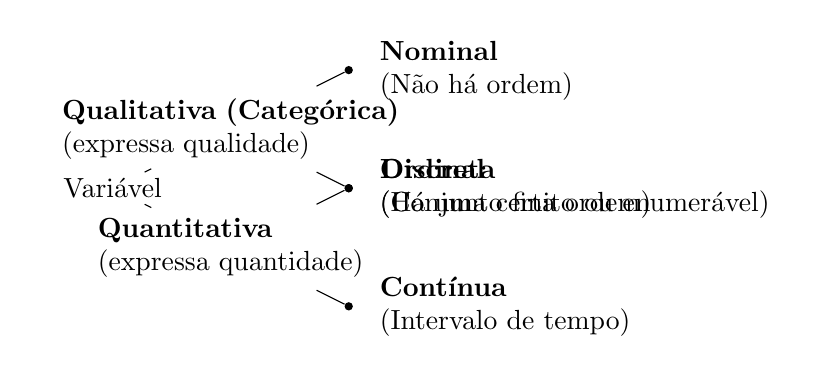
\begin{tikzpicture}[grow=right, sloped]
			\node[text width=4em, text centered] {Variável}
			child {
				node[text width=14em, text centered] {\begin{tabular}{l}\textbf{Quantitativa}\\(expressa quantidade)\end{tabular}}
				child {
					node[circle, minimum width=3pt,fill, inner sep=0pt, label=right:{\begin{tabular}{l}\textbf{Contínua}\\(Intervalo de tempo)\end{tabular}}] {}
				}
				child {
					node[circle, minimum width=3pt,fill, inner sep=0pt, label=right:{\begin{tabular}{l}\textbf{Discreta}\\(Conjunto finito ou enumerável)\end{tabular}}] {}
				}
			} child {
				node[text width=14em, text centered] {\begin{tabular}{l}\textbf{Qualitativa (Categórica)}\\(expressa qualidade)\end{tabular}}
				child {
					node[circle, minimum width=3pt, fill, inner sep=0pt, label=right:{\begin{tabular}{l}\textbf{Ordinal}\\(Há uma certa ordem)\end{tabular}}] {}
				}
				child {
					node[circle, minimum width=3pt,fill, inner sep=0pt, label=right:{\begin{tabular}{l}\textbf{Nominal}\\(Não há ordem)\end{tabular}}] {}
				}
			};
			\end{tikzpicture}
		}
	\end{pageWidthAreaPicture}
\end{pageWidthArea}

\begin{example}
	\label{example:estatistica_descritiva}
	
	Classifique as variáveis:
	\begin{enumerate}[label=\alph*)]
		\item \emphasis{Peso ou Altura:} variáveis do tipo peso ou altura são quantitativas, pois representam números e são contínuas pois o conjunto é não enumerável (quantitativa contínua).
		
		\item \emphasis{Número de tratores em uma propriedade rural:} é uma variável quantitativa pois representa um número e discreta pois seu conjunto é enumerável (quantitativa discreta).
		
		\item \emphasis{Uso do solo:} é uma variável qualitativa pois expressa uma qualidade e é nominal pois não há ordem nos possíveis valores (qualitativa nominal).
		
		\item \emphasis{Grau de Instrução:} é uma variável qualitativa pois expressa uma qualidade e ordinal pois há uma ordem nos possíveis valores (qualitativa ordinal).
	\end{enumerate}
\end{example}

\section{Representação Gráfica}

A representação gráfica tem por objetivo, dar ideia imediata dos resultados obtidos, permitindo ao leitor tirar conclusões sobre o comportamento da variável.

\subsection{Gráficos em colunas ou em barras}

Um exemplo de exibição de um mesmo gráfico, em formato de colunas e de barras pode ser visto na Figura \ref{picture:diversidade_coluna} e na Figura \ref{picture:diversidade_barra}, respectivamente.

\vspace{10pt}

\begin{pageWidthArea}
	\begin{pageWidthAreaPicture}{picture}{Diversidade de Cultivo de 36 Propriedades Rurais exibido em um Gráfico de Colunas.}
		\label{picture:diversidade_coluna}
		\centering
		\includegraphics[scale=0.4]{graphs/diversidade_cultivo}
	\end{pageWidthAreaPicture}
\end{pageWidthArea}

\vspace{10pt}

\begin{pageWidthArea}
	\begin{pageWidthAreaPicture}{picture}{Diversidade de Cultivo de 36 Propriedades Rurais exibido em um Gráfico de Barras.}
		\label{picture:diversidade_barra}
		\centering
		\includegraphics[scale=0.4]{graphs/diversidade_cultivo_barra}
	\end{pageWidthAreaPicture}
\end{pageWidthArea}

\subsection{Gráfico em setores}

\begin{sidepicture}{10pt}{table}{Dados sobre os domicílios particulares permanentes na cidade de Potirendaba - SP}
	\label{table:setores_domicilios}
	\begin{tabular}{lcc}\\\toprule
		\begin{tabular}{l}Imóvel\end{tabular}\vspace{10pt} & Domicílios & Ângulo \\ \midrule
		\begin{tabular}{l}Próprio\\já quitado\end{tabular}\vspace{10pt} & 2.135 & $186^{\text{o}}$\\
		\begin{tabular}{l}Próprio\\em aquisição\end{tabular}\vspace{10pt} & 872 & $76^{\text{o}}$\\ 
		\begin{tabular}{l}Alugado\end{tabular}\vspace{10pt} & 632 & $55^{\text{o}}$ \\ 
		\begin{tabular}{l}Cedido\end{tabular}\vspace{10pt} & 486 & $42^{\text{o}}$ \\
		\begin{tabular}{l}Outra forma\end{tabular}\vspace{10pt} & 9 & $1^{\text{o}}$ \\ \midrule
		\begin{tabular}{l}Total\end{tabular}\vspace{10pt} & 4.134 & $360^{\text{o}}$\\\bottomrule
	\end{tabular}
\end{sidepicture}

O gráfico em setores, também conhecido como gráfico de pizza, é muito utilizado para a exibição em porcentagem, onde, o ângulo de cada setor é dado por
\[
	x_i^{\text{o}}=\frac{360^{\text{o}}f_i}{n}\text{.}
\]

Um exemplo de gráfico de setores, criado a partir dos dados disponíveis na Tabela \ref{table:setores_domicilios}, pode ser visto na Figura \ref{picture:setores_domicilios}.

\vspace{160pt}

\begin{pageWidthArea}
	\begin{pageWidthAreaPicture}{picture}{Domicilios Particulares Permanentes em Potirendaba - SP Exibidos em um Gráfico de Setores.}
		\label{picture:setores_domicilios}
		\centering
		\includegraphics[scale=0.35]{graphs/domicilios}
	\end{pageWidthAreaPicture}
\end{pageWidthArea}

\newpage

\subsection{Gráfico em curvas ou linhas}

Um exemplo de gráfico em curva, também chamado de gráfico em linha, pode ser visto na Figura \ref{picture:linha_kw}.

\begin{pageWidthArea}
	\begin{pageWidthAreaPicture}{picture}{Demanda horária de quilowatt (KW) em um dia de pico de verão para um edifício comercial visualizado num gráfico em linha.}
		\label{picture:linha_kw}
		\centering
		\includegraphics[scale=0.35]{graphs/kw_linha}
	\end{pageWidthAreaPicture}
\end{pageWidthArea}

\subsection{Histograma}

Um histograma é uma representação gráfica de uma ditribuição de frequência por meio de retângulos justapostos. Um exemplo de histograma pode ser visto na Figura \ref{picture:histograma}.

\begin{pageWidthArea}
	\begin{pageWidthAreaPicture}{picture}{Tamanho de 80 Propriedades Rurais visto num Histograma.}
		\label{picture:histograma}
		\centering
		\includegraphics[scale=0.35]{graphs/histograma_rurais}
	\end{pageWidthAreaPicture}
\end{pageWidthArea}

\subsection{Curva Polida de Frequência}

Um exemplo de curva polida (suave) de frequência está na Figura \ref{picture:polida}.

\begin{pageWidthArea}
	\begin{pageWidthAreaPicture}{picture}{Tamanho de 80 Propriedades Rurais visto numa curva polida.}
		\label{picture:polida}
		\centering
		\includegraphics[scale=0.35]{graphs/polida}
	\end{pageWidthAreaPicture}
\end{pageWidthArea}

\newpage
\subsection{Histograma com Curva Polida de Frequência}

Um exemplo de histograma com curva polida (suave) de frequência está na Figura \ref{picture:polida_histograma}.

\begin{pageWidthArea}
	\begin{pageWidthAreaPicture}{picture}{Tamanho de 80 Propriedades Rurais visto numa curva polida junto com o histograma.}
		\label{picture:polida_histograma}
		\centering
		\includegraphics[width=\textwidth]{graphs/histograma_polida}
	\end{pageWidthAreaPicture}
\end{pageWidthArea}

\section{Medidas de Tendência Central e de Dispersão}

Os dados, apresentados em tabelas e gráficos, constituem a base de toda a informação. Mas, às vezes, é preciso resumir essa informação. Usam-se então as medidas de tendência central, que \emphasis{dão o(s) valor(es) em torno do qual os dados se distribuem}. Sabe-se, porém, que as medidas de tendência central são tanto mais apropriadas para descrever um conjunto de dados quanto \emphasis{menor for a dispersão}. Então, também é necessário e importante estudar as medidas de dispersão.

Dentre as medidas de "\emphasis{tendências centrais}" destacamos:
\begin{itemize}
	\item A média.
	\item A mediana.
	\item A moda.
\end{itemize}

Dentre as medidas de "\emphasis{dispersão} destacamos:
\begin{itemize}
	\item A amplitude.
	\item A variância.
	\item O desvio-padrão.
	\item O coeficiente de variação.
\end{itemize}

\subsection{Medidas de Tendência Central}

\subsubsection{Média Aritmética para Dados não Agrupados}

A média aritmética para dados não agrupados é o quociente da divisão da soma dos valores da variável pelo número total dos valores dessa variável.
\[
	\overline{x} = \frac{\displaystyle\sum_{i=1}^{n} x_i}{n}
	\text{,}
\]
onde $x_i$ são os valores da variável e $n$ é o número de valores dessa variável.

\begin{example}
	\label{example:pesos_bezerros}
	O peso ao nascer de 7 bezerros machos da raça Charolesa em quilogramas são os seguintes: 47, 34, 45, 28, 37, 40, 42. A média desses pesos é
	\[
		\overline{x}=\frac{47+34+45+28+37+40+42}{7}=39\text{,}
	\]
	logo a média dos pesos dos bezerros é de 39kg.
\end{example}

\subsubsection{Desvio em Relação à Média}

O desvio em relação à média é a diferença entre cada elemento de um conjunto de dados e a média aritmética, isto é,
\[
	d_i=x_i-\overline{x}\text{.}
\]

\begin{example}
	\label{example:pesos_bezerros_desvios}
	Do Exemplo \ref{example:pesos_bezerros}, tem-se os desvios, dados por $d_i=x_i-\overline{x}$,
	\begin{itemize}
		\item $d_1=47-39=8$.
		\item $d_2=34-39=-5$.
		\item $d_3=45-39=6$.
		\item $d_4=28-39=-11$.
		\item $d_5=37-39=-2$.
		\item $d_6=40-39=1$.
		\item $d_7=42-39=3$.
	\end{itemize}
\end{example}

A soma dos desvios em relação à média é sempre nula. Do Exemplo \ref{example:pesos_bezerros_desvios}, tem-se
\[
	\sum_{i=1}^{7}d_i = 8-5+6-11-2+1+3=0\text{.}
\]

\begin{theorem}
	Somando-se (ou subtraindo-se) uma constante $c$ de todos os valores de um conjunto de dados, a média desse novo conjunto de dados fica aumentada (ou diminuída) dessa contante. Ou seja, se
	\[
		y_i=x_i\pm c\text{,}
	\]
	tem-se que
	\[
		\overline{y}=\overline{x}\pm c\text{.}
	\]
\end{theorem}

\begin{example}
	Somando uma constante 2 a cada um dos valores do conjunto de dados do Exemplo \ref{example:pesos_bezerros}, tem-se um novo conjunto dado por: 49, 36, 47, 30, 39, 42 e 44, e uma nova média dada por
	\[
		\overline{y}=\frac{49+36+47+30+39+42+44}{7}=41\text{.}
	\]
	
	Assim, vale que
	\[
		\overline{y}=\overline{x}+2=39+2=41\text{,}
	\]
	Ou seja, a nova média é 41 kg.
\end{example}

\begin{theorem}
	Multiplicando-se (ou dividindo-se) todos os valores de um conjunto de dados por uma constante $c$, a média desse novo conjunto de dados fica multiplicada (ou dividida) por essa constante. Ou seja, se
	\[
		y_i=x_i\cdot c\text{,}
	\]
	então, tem-se
	\[
		\overline{y}=\overline{x}\cdot c\text{.}
	\]
	
	Ainda, se
	\[
		y_i=\frac{x_i}{c}\text{,}
	\]
	tem-se
	\[
		\overline{y}=\frac{\overline{x}}{c}\text{.}
	\]
\end{theorem}

\begin{example}
	Multiplicando por 3 cada um dos valores do conjunto de dados do Exemplo \ref{example:pesos_bezerros}, tem-se um novo conjunto dado por: 141, 102, 135, 84, 111, 120 e 126 e uma nova média dada por
	\[
		\overline{y}=\frac{141+102+135+84+111+120+126}{7}=117\text{.}
	\]
	
	Assim, tem-se que
	\[
		\overline{y}=\overline{x}\cdot 3=39\cdot 3=117
		\text{,}
	\]
	portanto, a nova média é de 117 kg.
\end{example}

\subsubsection{Média Aritmética para Dados Agrupados Sem Intervalo de Classe}

Neste caso, como as frequências $f_i$ são números indicadores da intensidade de cada valor da variável, elas funcionam como fatores de ponderação, o que nos leva a calcular a \emphasis{média aritmética ponderada}, dada por
\[
	\overline{x}=\frac{
		\displaystyle \sum_{i=1}^{k} x_i f_i
	}{
		\displaystyle \sum_{i=1}^{n} f_i
	}
	= \frac{
		\displaystyle \sum_{i=1}^{k} x_i f_i
	}{
		n
	}
	\text{,}
\]
onde $k$ é o número de classes.

\begin{sidepicture}{10pt}{table}{Vendas de um determinado produto de um supermercado (R\$)}
	\label{table:exemplo_vendas_produto}
	\begin{tabular}{lcc}\\\toprule
		Preço ($x_i$) & Frequência ($f_i$) & $x_i\cdot f_i$ \\ \midrule
		9 & 2 & 18 \\
		10 & 5 & 50 \\
		11 & 3 & 33 \\ \midrule
		Total ($\Sigma$) & 10 & 101 \\ \bottomrule
	\end{tabular}
\end{sidepicture}

\begin{example}
	Durante a semana, um supermercado vendeu determinado produto pelos preços da Tabela \ref{table:exemplo_vendas_produto}. O preço médio pode ser determinado por
	\[
		\overline{x} = \frac{
			\displaystyle\sum_{i=1}^{3} x_i f_i
		}{
			\displaystyle\sum_{i=1}^{3} f_i
		}
		=
		\frac{101}{10}
		=10,10\text{.}
	\]
	
	Desse modo, o preço médio desse produto nessa semana no supermercado é de R\$ 10,10.
\end{example}

\subsubsection{Média Aritmética para Dados Agrupados com Intervalo de Classe}

Neste caso, "\emphasis{convencionamos}" que todos os valores incluídos em um determinado intervalo de classe sejam representados pelo seu \emphasis{ponto médio} ($x^{*}$), e determinamos a média aritmética ponderada através de:
\[
	\overline{x}=\frac{	
		\displaystyle \sum_{i=1}^{k} x_i^{*} f_i
	}{
		\displaystyle \sum_{i=1}^{k} f_i
	}
	= \frac{
		\displaystyle \sum_{i=1}^{k} x_i^{*} f_i
	}{
		n
	}
	\text{,}
\]
onde $k$ é o número de classes.

\begin{pageWidthArea}
	\begin{pageWidthAreaPicture}{table}{Aluguel das residências gerenciadas por um imobiliária}
		\label{table:exemplo_aluguel_residencias}
		\hspace{-15pt}
		\resizebox{\textwidth}{!}{%
			\begin{tabular}{lccc}\\\toprule
				Aluguel (R\$) ($x_i$) & Residências ($f_i$) & Ponto médio ($x^{*}$) & $x_i\cdot f_i$ \\ \midrule
				\hspace{11pt}0 $\vdash$ 200 & 30 & 100 & 3.000 \\
				200 $\vdash$ 400 & 52 & 300 & 15.600 \\
				400 $\vdash$ 600 & 28 & 500 & 14.000 \\ 
				600 $\vdash$ 800 & 7 & 700 & 4.900 \\
				800 $\vdash$ 1.000 & 3 & 900 & 2.700\\\midrule
				Total & 120 & - & 40.200 \\ \bottomrule
			\end{tabular}
		}
	\end{pageWidthAreaPicture}
\end{pageWidthArea}

\begin{example}
	Uma imobiliária gerencia o aluguel de residências particulares, conforme a Tabela \ref{table:exemplo_aluguel_residencias}. A média dos aluguéis gerenciados por esta imobiliária pode ser cálculada como
	\[
		\overline{x}=\frac{
			\displaystyle\sum_{i=1}^{5} x_{i}^{*} f_i
		}{
			\displaystyle\sum_{i=1}^{5} f_i
		}
		= \frac{40.200}{120}
		= 335\text{.}
	\]
	
	Portanto, a média dos aluguéis dessa imobiliária é de R\$ 335,00.
\end{example}

\subsection{Mediana}

A mediana é o \emphasis{valor central} que divide um conjunto de "\emphasis{dados ordenados}" ao meio, deixando 50\% dos valores dos dados a sua esquerda e 50\% à sua direita.

\begin{example}
	\label{example:mediana_vendedor}
	O departamento de recursos humanos de uma empresa, tendo em vista o aumento de produtividade de seus vendedores, resolveu, premiar com um aumento de 5\% no salário, a metade de seus vendedores mais eficientes. Para isto, fez um levantamento de vendas semanais (em milhares de reais), por vendedor, obtendo os dados: 22, 18, 24, 19, 20, 21, 28, 26 e 25. A partir de qual volume de vendas o vendedor será premiado?
	
	O Rol dos conjuntos de dados é
	\begin{center}
		18, 19, 20, 21, \emphasis{22}, 24, 25, 26, 28\text{,}
	\end{center}
	que é uma sequência ímpar, portanto, a mediana é $md=R\$\text{ }22.000,00$. Assim o vendedor será premiado se o seu volume de vendas for a partir de R\$ 22.000,00.
\end{example}

\begin{example}
	No Exemplo \ref{example:mediana_vendedor}, considere, agora, que temos mais um vendedor nesta empresa, com um volume de vendas (em milhares de reais) de 23. Então, tem-se o Rol
	\begin{center}
		18, 19, 20, 21, \emphasis{22}, \emphasis{23}, 24, 25, 26, 28,
	\end{center}
	que é uma sequência ímpar e, portanto, a mediana é calculada pela média entre os valores centrais,
	\[
		md=\frac{22 + 23}{2}=22,5\text{,}
	\]
	ou seja, o vendedor agora será premiado se o seu volume de vendas for a partir de R\$ 22.500,00.
\end{example}

\subsection{Moda}

Denominamos por moda o valor que ocorre com maior frequência em um conjunto de dados.

\begin{example}
	Os dados abaixo se referem ao consumo em kg, de um produto colocado em oferta, limitado a 5 kg no máximo por cliente.
	\begin{center}
		\emphasis{3}, 1, 2, 5, \emphasis{3}, 4, \emphasis{3} e 2.
	\end{center}
	
	A moda para o consumo desse produto é $mo=3$ kg, pois o valor 3 é o que mais ocorre.
\end{example}

\begin{example}
	Um grupo de funcionários teve seus pesos anotados:
	\begin{center}
		82, 73, 61, 58, 88, 77, 64 e 56.
	\end{center}
	
	Neste caso, não existe moda, pois todos os valores ocorrem com a mesma frequência.
\end{example}

\begin{example}
	As alturas de oito pessoas são medidas para fins de estudos. Suas alturas são:
	\begin{center}
		\emphasis{1,72}; 1,84; \textbf{1,64}; 1,76; \emphasis{1,72}; 1,58; \textbf{1,64} e 1,81.
	\end{center}
	
	Portanto, a moda é 1,64 m e 1,72 m, pois os valores 1,64 e 1,72 são os valores que mais ocorreram.
\end{example}

\subsection{Qual a Melhor Medida de Centralidade?}

Não há uma única melhor resposta para esta questão, porque não há critérios objetivos para a determinação da medida mais representativa para todos os conjuntos de dados. As diferentes medidas de centralidade tem diferentes vantagens e desvantagens, algumas das quais estão resumidas no Quadro \ref{quadro:comparacao_medida_tc}.\\

\begin{pageWidthArea}
	\begin{pageWidthAreaPicture}{frame}{Comparação entre as medidas de tendências centrais.}
		\label{quadro:comparacao_medida_tc}
		\hspace{-15pt}
		\resizebox{\textwidth}{!}{%
		\begin{tabular}{|c|c|c|c|c|c|}
			\hline
			Medida & Uso & Existência & \begin{tabular}[c]{@{}c@{}}Leva em\\conta todos\\os valores\end{tabular} & \begin{tabular}[c]{@{}c@{}}Afetada\\por\\Outliers\end{tabular} & Vantagens\\ \hline
			Média & "Exagerado" & Sempre & Sim & Sim & \begin{tabular}[c]{@{}c@{}}Funciona bem\\com muitos\\métodos\\estatísticos.\end{tabular}\\ \hline
			Mediana & Comumente & Sempre & Não & Não & \begin{tabular}[c]{@{}c@{}}Sempre uma\\boa escolha\\na presença\\de \textit{outliers}.\end{tabular}\\ \hline
			Moda & Raramente & \begin{tabular}[c]{@{}c@{}}Pode não\\existir ou ter\\mais de uma\end{tabular} & Não & Não & \begin{tabular}[c]{@{}c@{}}Apropriada\\para dados\\nominais.\end{tabular}\\ \hline
		\end{tabular}
		}
	\end{pageWidthAreaPicture}
\end{pageWidthArea}

\begin{remark}
	Para um conjunto de dados unimodal que é aproximadamente simétrico, a média, a mediana e a moda são muito próximas.
\end{remark}

\begin{remark}
	Para um conjunto de dados obviamente assimétrico, seria melhor informar tanto a média como a mediana.
\end{remark}

\begin{pageWidthArea}
	\begin{pageWidthAreaPicture}{table}{Distribuição de números de fregueses de um restaurante italiano}
		\label{table:exemplo_restaurante_italiano}
		\hspace{-15pt}
		\resizebox{\textwidth}{!}{%
			\begin{tabular}{cccccccc}\\\toprule
				Dias & Seg. & Ter. & Qua. & Qui. & Sex. & \textbf{Sab.} & Dom \\ \midrule
				Fregueses & 24 & 21 & 28 & 31 & 42 & \emphasis{226} & 39 \\ \bottomrule
			\end{tabular}
		}
	\end{pageWidthAreaPicture}
\end{pageWidthArea}

\begin{example}
	Um restaurante "Italiano" recebeu em uma determinada semana, uma certa quantidade de fregueses, e sabe-se que sábado foi um dia atípico pois chegaram ao restaurante três turmas de turistas. Os dados estão condensados na Tabela \ref{table:exemplo_restaurante_italiano}. A fim de ajudar o dono do restaurante, resuma esses dados em uma medida de tendência central mais apropriada.
	
	O rol do conjunto de dados é
	\begin{center}
		21, 24, 28, 31, 39, 42, \emphasis{226},
	\end{center}
	cuja média é 59 fregueses e a mediana é de 31 fregueses. A medida de tendência central mais "apropriada" é a mediana, pois esta representa melhor o conjunto de dados.
\end{example}

\begin{pageWidthArea}
	\begin{pageWidthAreaPicture}{table}{Intenção de compra segundo os maridos}
		\label{table:exemplo_compras_marido}
		\resizebox{\textwidth}{!}{%
			\begin{tabular}{cccccc}\\\toprule
				Marido & 1 & 2 & 3 & 4 & 5 \\ \midrule
				Presente & Roupa & Flores & CD & Livro & \emphasis{Carro}\\ \midrule
				R\$ & 60,00 & 50,00 & 44,00 & 48,00 & \emphasis{25.000,00}\\ \bottomrule
			\end{tabular}
		}
	\end{pageWidthAreaPicture}
\end{pageWidthArea}

\begin{example}
	Numa pesquisa de consumo para o Natal, cinco maridos responderam o que e quanto eles pretendiam gastar com o presente para suas respectivas esposas. Os dados estão na Tabela \ref{table:exemplo_compras_marido}. O Rol do conjunto de dados é
	\begin{center}
		44,00; 48,00; \textbf{50,00}; 60,00; \emphasis{25.000,00}.
	\end{center}
	Neste caso, a mediana é "muito mais apropriada" do que a média para representar esse conjunto de dados, pois a mediana é R\$ 50,00 e a média é R\$ 5.040,40.
\end{example}

\section{Medidas de Dispersão}

\subsection{Amplitude Total}

A amplitude total é a diferença entre os valores extremos do conjunto de dados.

\begin{example}
	A produção diária de álcool na usina A durante uma semana foi de: 10, 14, 13, 15, 16 e 18 mil litros. Determine a amplitude total.
	\[
		A_t=18-10=8\text{,}
	\]
	assim, a amplitude total é de 8 mil litros.
\end{example}

\begin{remark}
	Dois conjuntos de dados podem ter dispersão diferentes e apresentar a mesma amplitude total.
\end{remark}

\begin{example}
	Considere os dados de produção diária de álcool da usina B durante uma semana: 7, 15, 14, 15, 14, 15 mil litros. A amplitude total é 
	\[
		A_t = 15 - 7 = 8\text{,}
	\]
	ou seja, 8 mil litros.
\end{example}

Considerando os dois exemplos, a amplitude da produção diária de álcool é a mesma para as duas usinas, porém, a usina B tem menor dispersão em relação a A.

Embora a amplitude total seja a medida de dispersão mais simples, existem várias restrições ao seu uso devido a sua instabilidade, uma vez que, ela utiliza somente os valores extremos do conjunto de dados, sendo extremamente sensível à presença de valores extremos (outliers). Neste caso, precisamos de uma medida que foge a essa "falha", isto é, que leva em consideração todos os valores de um conjunto de dados.

\subsection{Variância}

A variância é uma medida de variação de todos os valores de um conjunto de dados em torno de sua média, calculadas por
\begin{equation}
	\label{eqn:variancia_populacao}
	\sigma ^2 = \frac{
		\displaystyle \sum_{i=1}^{n} (x_i - \overline{x})^2
	} {
		n
	} \text{.}
\end{equation}

Desse modo, a variância é definida como a soma dos quadrados dos desvios, dividida por $n$. A Fórmula \ref{eqn:variancia_populacao} é chamada de \emphasis{Variância para População}.

Prova-se, no entanto, que para ter propriedades estatísticas desejáveis, é preciso que ese valor seja multiplicado pelo fator de correção
\[
	\frac{n}{n-1}
	\text{.}
\]

Dessa forma, a variância pode ser reescrita como
\begin{equation}
	\label{eqn:variancia_amostras}
	S^2=\frac{
		\displaystyle \sum_{i=1}^{n} (x_i - \overline{x})^2
	} {
		n-1
	}\text{.}
\end{equation}

A Fórmula \ref{eqn:variancia_amostras} é chamada de \emphasis{Variância para Amostras}. É possível desenvolver essa fórmula, algebricamente, de onde tira-se que
\[
	S^2=\frac{
		\displaystyle \sum_{i=1}^{n} x_i^2
		-
		\displaystyle \frac{
			\left (
				\displaystyle \sum_{i=1}^{n} x+i
			\right ) ^2
		}{n}
	} {
		n-1
	}
	\text{.}
\]

\begin{example}
	\label{example:sinistros_var}
	Uma corretora de seguros analisou o número de sinistros de cinco de seus clientes: 0, 1, 2, 3 e 4. 
	
	Para o cálculo da variância desses dados, pode-se fazer com passos intermediários, como, por exemplo, somar todos os números e, ainda, somar todos os seus quadrados. Representaremos aqui, como $\sum x_i=0+1+2+3+4=10$ e $\sum x_i^2= 0^2+1^2+2^2+3^2+4^2=30$. Deste modo,
	\[
		S^2=\frac{
			\displaystyle\sum_{i=1}^{n} x_i^2
			-
			\displaystyle\frac{
				\left (
					\displaystyle \sum_{i=1}^{n} x_i
				\right )^2
			}{n}
		}{n-1}
		=\frac{30-\displaystyle\frac{(10)^2}{5}}{5-1}
		=\frac{10}{4}
		=2,5\text{,}
	\]
	portanto a variância é de 2,5 sinistros$^2$.
\end{example}


A variância tem a desvantagem de apresentar unidade de medida igual ao quadrado da unidade de medida dos dados. Dessa forma surge a necessidade de se extrair a raiz quadrada da variância, definindo assim o \emphasis{Desvio-Padrão}.

\subsection{Desvio-Padrão}

O desvio-padrão é a raiz quadrada positiva da variância. O desvio-padrão tem a vantagem de ter a mesma unidade de  medida dos dados.

\begin{example}
	No Exemplo \ref{example:sinistros_var}, tem-se que a variância é de 2,5 sinistros$^2$, então o desvio-padrão (S) será dado por
	\[
		S=\sqrt{2,5}=1,58\text{ sinistros.}
	\]
\end{example}

\begin{theorem}
	Somando-se (ou subtraindo-se) uma constante $c$ de todos os valores de um conjunto de dados, o desvio-padrão não se altera. Isto é, se
	\[
		y_i=x_i\pm c\text{,}
	\]
	então,
	\[
		S_y=S_x\text{.}
	\]
\end{theorem}

\begin{theorem}
	Multiplicando-se todos os valores de um conjunto de dados por uma constante $c\neq 0$, o desvio-padrão fica multiplicado por essa constante. Isto é, se
	\[
		y_i=x_i\cdot c\text{,}
	\]
	então,
	\[
		S_y=c\cdot S_x\text{.}
	\]
\end{theorem}

Tanto a variância quanto o desvio padrão são medidas que fornecem informações complementares à informação contida na média.

\begin{pageWidthArea}
	\begin{pageWidthAreaPicture}{table}{Tempo de espera em filas do "Banco Magnífico"}
		\label{table:banco_magnifico}
		% TODO: insert hspace negative
		\resizebox{\textwidth}{!}{%
			\begin{tabular}{@{}cccccccccc@{}} \toprule
				Sistema de Fila & \multicolumn{8}{c}{Tempo de Espera (min)} & Média \\ \midrule
				Fila Única      & 4  & 9  & 9  & 10  & 10  & 11  & 11  & 12 & 10    \\
				Filas Separadas & 5  & 6  & 8  & 10  & 10  & 13  & 14  & 14 & 10    \\ \bottomrule
			\end{tabular}
		}
	\end{pageWidthAreaPicture}
\end{pageWidthArea}

\begin{example}
	O "Banco Magnífico" ainda adota o sistema de filas separadas para cada caixa. Os diretores do banco afirmam que o tempo médio de espera será igual, se trocarem o sistema atual para uma única fila, pois, a configuração da fila não afetará a eficiência dos atendentes. No entanto, resolveram fazer uma experiência. Baseados nos dados da Tabela \ref{table:banco_magnifico}, que decisão você tomaria?
	
	A variância para o sistema de fila única é de
	\[
		S_U^2 = \frac{
			\displaystyle\sum_{i=1}^{n} x_i^2 -
			\displaystyle\frac{
				\left (
					\displaystyle\sum_{i=1}^{n} x_i
				\right ) ^ 2
			}{n}
		}{n-1}
		=
		\frac{812-\displaystyle\frac{(80)^2}{8}}{8-1}
		=\frac{12}{7}
		=1,71\text{,}
	\]
	e o desvio-padrão é dado por
	\[
		S_{U} = \sqrt{\frac{12}{7}}=1,31\text{ min.}
	\]
	
	Para o sistema de filas separadas tem-se a variância de
	\[
		S_S^2 = \frac{
			\displaystyle\sum_{i=1}^{n} x_i^2 -
			\displaystyle\frac{
				\left (
					\displaystyle\sum_{i=1}^{n} x_i
				\right ) ^ 2
			}{n}
		}{n-1}
		=
		\frac{886-\displaystyle\frac{(80)^2}{8}}{8-1}
		=\frac{86}{7}
		=12,29\text{,}
	\]
	com desvio-padrão de
	\[
		S_S=\sqrt{\frac{86}{7}}=3,51\text{ min.}
	\]
	
	Portanto, é preferível utilizar o sistema de fila única, pois este se apresenta mais "confiável" em relação ao tempo de espera, quando comparado ao sistema de filas separadas.
\end{example}

\section{Teorema de Chebyshev}

A proporção de qualquer conjunto de dados que se situa a $k$ desvios padrões da média é sempre, no mínimo, $1-\frac{1}{k^2}$, onde $k$ é qualquer número positivo maior do que 1. Para $k=2$ e $k=3$, obtemos as seguintes afirmativas:

\begin{enumerate}
	\item Pelo menos 3/4 (ou 75\%) de todos os valores do conjunto de dados, localizam-se a 2 desvios padrões da média.
	
	\item Pelo menos 8/9 (ou 89\%) de todos os valores do conjunto de dados, localizam-se a 3 desvios padrões da média.
\end{enumerate}

\begin{example}
	Os escores QI de adultos normais no teste Weschler tem uma média de 100 e desvio-padrão de 15. O que podemos concluir do teorema de Chebyshev?
	
	\begin{enumerate}
		\item Ao menos 75\% de todos os adultos tem escores QI a 2 desvios padrões da média, ou seja, entre 70 e 130.
		
		\item Ao menos 89\% de todos os adultos tem escores QI a 3 desvios padrões da média, ou seja, entre 55 e 145.
	\end{enumerate}
\end{example}

\section{Coeficiente de Variação (Pearson)}

É uma medida de dispersão, que tem por finalidade comparar conjuntos de dados \emphasis{não homogêneos} e, em geral, de \emphasis{grandezas diferentes}. O coeficiente de variação de um conjunto de dados é indicado por CV e definido por:
\begin{equation}
	CV=\frac{S}{\overline{x}}\text{,}
\end{equation}
ou
\begin{equation}
	CV=\frac{S}{\overline{x}}\cdot 100\text{.}
\end{equation}

O coeficiente de variação de Pearson é um número adimensional.

Uma classificação do coeficiente de variação é
\begin{itemize}
	\item $0\%\leqslant CV < 10\%$: \emphasis{Variação Baixa};
	\item $10\%\leqslant CV < 20\%$: \emphasis{Variação Média};
	\item $20\%\leqslant CV < 30\%$: \emphasis{Variação Alta};
	\item $CV \geqslant 30$: \emphasis{Variação Muito Alta}.
\end{itemize}

Em geral, quando comparamos dispersões, ocorrem três situações:

\begin{enumerate}
	\item Os conjuntos de dados têm a mesma grandeza, e suas médias são muito próximas. Nesse caso, o coeficiente de variação (CV) não traz muito mais informação do que o desvio padrão (Tabela \ref{table:cv_caso1}).
	
	\item Os conjuntos de dados têm a mesma grandeza, mas suas médias são "significantemente" diferentes (Tabela \ref{table:cv_caso2}).
	
	\item Os conjuntos de dados têm grandezas diferentes. Neste caso o uso do coeficiente de variação se torna "muito viável" na comparação dos conjuntos, uma vez que o uso do desvio-padrão é inviável (Tabela \ref{table:cv_caso3}).
\end{enumerate}

\begin{pageWidthArea}
	\begin{pageWidthAreaPicture}{table}{Coeficiente de variação para a duração de duas marcas de pneus}
		\label{table:cv_caso1}
		\resizebox{\textwidth}{!}{%
			\begin{tabular}{cccc}\\\toprule
				Duração & Média & Desvio-Padrão & CV \\ \midrule
				Rodabem & 31.000 km & 3.500 km & 11,29\% \\
				Duratex & 30.000 km & 3.200 km & 10,67\% \\ \bottomrule
			\end{tabular}
		}
	\end{pageWidthAreaPicture}
\end{pageWidthArea}

\begin{pageWidthArea}
	\begin{pageWidthAreaPicture}{table}{Coeficiente de variação para o tempo de serviço nos últimos empregos}
		\label{table:cv_caso2}
		\resizebox{\textwidth}{!}{%
			\begin{tabular}{cccc}\\\toprule
				Grupo & Média & Desvio-Padrão & CV \\ \midrule
				João & 2,1 anos & 0,87 anos & 41,43\% \\
				Lucas & 2,6 anos & 1,01 anos & 38,85\% \\ \bottomrule
			\end{tabular}
		}
	\end{pageWidthAreaPicture}
\end{pageWidthArea}

\begin{pageWidthArea}
	\begin{pageWidthAreaPicture}{table}{Coeficiente de variação para altura e peso dos funcionários da empresa Avante \& Avante}
		\label{table:cv_caso3}
		\resizebox{\textwidth}{!}{%
			\begin{tabular}{cccc}\\\toprule
				Funcionários & Média & Desvio-Padrão & CV \\ \midrule
				Altura & 1,69 m & 0,11 m & 6,51\% \\
				Peso & 64,8 kg & 5,23 kg & 8,07\% \\ \bottomrule
			\end{tabular}
		}
	\end{pageWidthAreaPicture}
\end{pageWidthArea}

\section{Medidas Separatrizes}

\subsection{Quartis}

Os quartis dividem o conjunto de dados em quatro partes iguais. Assim, tem-se
\begin{itemize}
	\item \emphasis{$Q_1$}: O primeiro quartil, que separa o conjunto de dados deixando 25\% de seus valores à esquerda e 75\% à direita.
	\item \emphasis{$Q_2$}: O segundo quartil, que coincide com a mediana, isto é, divide o conjunto de dados ao meio.
	\item \emphasis{$Q_3$}: O terceiro quartil, que separa o conjunto de dados deixando 75\% de seus valores à esquerda e 25\% à direita.
\end{itemize}

\subsection{Percentis}

Os percentis dividem o conjunto de dados em 100 partes iguais. Assim, tem-se
\begin{itemize}
	\item \emphasis{$P_1$}: Primeiro percentil, que separa o conjunto de dados deixando 1\% de seus valores à esquerda e 99\% à direita.
	\item \emphasis{$P_2$}: Segundo percentil, que separa o conjunto de dados deixando 2\% de seus valores à esquerda e 98\% à direita.
	\begin{center}
		$\vdots$
	\end{center}
	\item \emphasis{$P_{99}$}: 99$^{\text{o}}$ percentil, que separa o conjunto de dados deixando 99\% de seus valores à esquerda e 1\% à direita.
\end{itemize}

\begin{remark}
	É importante notar que $Q_1=P_{25}$, $Q_2=P_{50}$ e $Q_3=P_{75}$.
\end{remark}

\subsection{Aproximação para o Cálculo dos Percentis}

Considerando o número
\[
\frac{i\cdot n}{100}\text{,}
\]
tem-se dois casos:
\begin{itemize}
	\item Se $\frac{i\cdot n}{100}$ é um número inteiro, então $P_i$ é um dos elementos do conjunto de dados.
	
	\item Se $\frac{i\cdot n}{100}$ não é um número inteiro, então $P_i$ é a média entre o valor aproximado por falta e por excesso.
\end{itemize}

\begin{example}
	Dados os números de horas de trabalho perdidas por dia em uma lavoura devido a incidentes relacionados ao clima: 2, 5, 8, 5, 5, 10, 1, 8, 12, 9, 12 e 11. Determine o primeiro quartil.
	
	Como $Q_1=P_{25}$, logo, basta calcular $P_{25}$, ou seja, se $i=25$ e $n=12$, logo tem-se $\frac{i\cdot n}{100}=\frac{25\cdot 12}{100}=3$, portanto, $P_{25}$ é o terceiro elemento do rol desse conjunto de dados:
	\begin{center}
		1, 2, \emphasis{5}, 5, 5, 8, 8, 9, 10, 11, 12, 12\text{,}
	\end{center}
	portanto, $Q_1=5$ horas/dia.
\end{example}

\begin{example}
	Considere o seguinte conjunto de dados, em kg, referentes ao peso de bovinos com uma determinada idade: 265, 197, 346, 280, 268, 200, 221, 261. Calcule o percentil de ordem 60.
	
	Chamando $i=60$ e $n=80$, tem-se $\frac{i\cdot n}{100}=\frac{60\cdot 8}{100}=4,8$, portanto, $P_{60}$ será a média entre o 4$^{\text{o}}$ e o 5$^{\text{o}}$ elementos do rol desses dados:
	\begin{center}
		197, 200, 221, \emphasis{261}, \emphasis{265}, 268, 280, 346\text{,}
	\end{center}
	de onde,
	\[
		P_{60}=\frac{261 + 265}{2}=263\text{,}
	\]
	isto é, $P_{60}=263$ kg.
\end{example}

\section{Gráfico Box-Plot}

O gráfico box-plot é uma representação gráfica envolvendo os quartis. Definimos uma "caixa" com o nível superior dado pelo terceiro quartil e o nível inferior pelo primeiro quartil. A mediana é representada por um traço no interior da caixa e segmentos de reta são colocados da caixa até os valores extremos, caso os valores extremos estiverem no máximo até $1,5\cdot DQ$ da caixa, onde
\[
DQ=Q_3-Q_1\text{,}
\]
distância chamada de diferença interquartílica. 

\begin{example}
	Considerando o conjunto de dados: 1, 2, 2, 3, 4, 4, 5 e 8 é possível construir um gráfico box-plot a partir dos dados conhecidos, como se pode ver na Figura \ref{picture:ex_boxplot}.
\end{example}

\newpage

\begin{pageWidthArea}
	\begin{pageWidthAreaPicture}{picture}{Boxplot aaaaaa.}
		\label{picture:ex_boxplot}
		\centering
		\resizebox{\textwidth}{!}{%
			\includegraphics[width=\textwidth]{boxplot/box_plot_01}
		}
	\end{pageWidthAreaPicture}
\end{pageWidthArea}
